% Formatting: https://github.com/gillescastel/lecture-notes/

\documentclass{report}
% basics
\usepackage[utf8]{inputenc}
\usepackage[T1]{fontenc}
\usepackage{textcomp}
\usepackage[english]{babel}
\usepackage{url}
% \usepackage{hyperref}
% \hypersetup{
%     colorlinks,
%     linkcolor={black},
%     citecolor={black},
%     urlcolor={blue!80!black}
% }
\usepackage{graphicx}
\usepackage{float}
\usepackage{booktabs}
\usepackage[shortlabels]{enumitem}
% \usepackage{parskip}
\usepackage{emptypage}
\usepackage{subcaption}
\usepackage{multicol}
\usepackage[usenames,dvipsnames]{xcolor}

% \usepackage{cmbright}


\usepackage{amsmath, amsfonts, mathtools, amsthm, amssymb}
\usepackage{mathrsfs}
\usepackage{cancel}
\usepackage{blindtext}
\usepackage{bm}
\newcommand\N{\ensuremath{\mathbb{N}}}
\newcommand\R{\ensuremath{\mathbb{R}}}
\newcommand\Z{\ensuremath{\mathbb{Z}}}
\renewcommand\O{\ensuremath{\emptyset}}
\newcommand\Q{\ensuremath{\mathbb{Q}}}
\newcommand\C{\ensuremath{\mathbb{C}}}
\DeclareMathOperator{\sgn}{sgn}
\usepackage{systeme}
\let\svlim\lim\def\lim{\svlim\limits}
\let\implies\Rightarrow
\let\impliedby\Leftarrow
\let\iff\Leftrightarrow
\let\epsilon\varepsilon
\usepackage{stmaryrd} % for \lightning
\newcommand\contra{\scalebox{1.1}{$\lightning$}}
% \let\phi\varphi





% correct
\definecolor{correct}{HTML}{009900}
\newcommand\correct[2]{\ensuremath{\:}{\color{red}{#1}}\ensuremath{\to }{\color{correct}{#2}}\ensuremath{\:}}
\newcommand\green[1]{{\color{correct}{#1}}}



% horizontal rule
\newcommand\hr{
    \noindent\rule[0.5ex]{\linewidth}{0.5pt}
}


% hide parts
\newcommand\hide[1]{}



% si unitx
\usepackage{siunitx}
\sisetup{locale = FR}
% \renewcommand\vec[1]{\mathbf{#1}}
\newcommand\mat[1]{\mathbf{#1}}


% tikz
\usepackage{tikz}
\usepackage{tikz-cd}
\usetikzlibrary{intersections, angles, quotes, calc, positioning}
\usetikzlibrary{shapes,arrows}
\usetikzlibrary{arrows.meta}
\usepackage{pgfplots}
\pgfplotsset{compat=1.13}


\tikzset{
    force/.style={thick, {Circle[length=2pt]}-stealth, shorten <=-1pt}
}

% theorems
\usepackage{thmtools}
\usepackage[framemethod=TikZ]{mdframed}
\mdfsetup{skipabove=1em,skipbelow=0em, innertopmargin=5pt, innerbottommargin=6pt}


\theoremstyle{definition}

\makeatletter


\@ifclasswith{report}{nocolor}{
    \declaretheoremstyle[headfont=\bfseries\sffamily, bodyfont=\normalfont, mdframed={ nobreak } ]{thmgreenbox}
    \declaretheoremstyle[headfont=\bfseries\sffamily, bodyfont=\normalfont, mdframed={ nobreak } ]{thmredbox}
    \declaretheoremstyle[headfont=\bfseries\sffamily, bodyfont=\normalfont]{thmbluebox}
    \declaretheoremstyle[headfont=\bfseries\sffamily, bodyfont=\normalfont]{thmblueline}
    \declaretheoremstyle[headfont=\bfseries\sffamily, bodyfont=\normalfont, numbered=no, mdframed={ rightline=false, topline=false, bottomline=false, }, qed=\qedsymbol ]{thmproofbox}
    \declaretheoremstyle[headfont=\bfseries\sffamily, bodyfont=\normalfont, numbered=no, mdframed={ nobreak, rightline=false, topline=false, bottomline=false } ]{thmexplanationbox}
    \AtEndEnvironment{eg}{\null\hfill$\diamond$}%
}{
    \declaretheoremstyle[
        headfont=\bfseries\sffamily\color{ForestGreen!70!black}, bodyfont=\normalfont,
        mdframed={
            linewidth=2pt,
            rightline=false, topline=false, bottomline=false,
            linecolor=ForestGreen, backgroundcolor=ForestGreen!5,
        }
    ]{thmgreenbox}

    \declaretheoremstyle[
        headfont=\bfseries\sffamily\color{NavyBlue!70!black}, bodyfont=\normalfont,
        mdframed={
            linewidth=2pt,
            rightline=false, topline=false, bottomline=false,
            linecolor=NavyBlue, backgroundcolor=NavyBlue!5,
        }
    ]{thmbluebox}

    \declaretheoremstyle[
        headfont=\bfseries\sffamily\color{NavyBlue!70!black}, bodyfont=\normalfont,
        mdframed={
            linewidth=2pt,
            rightline=false, topline=false, bottomline=false,
            linecolor=NavyBlue
        }
    ]{thmblueline}

    \declaretheoremstyle[
        headfont=\bfseries\sffamily\color{RawSienna!70!black}, bodyfont=\normalfont,
        mdframed={
            linewidth=2pt,
            rightline=false, topline=false, bottomline=false,
            linecolor=RawSienna, backgroundcolor=RawSienna!5,
        }
    ]{thmredbox}

    \declaretheoremstyle[
        headfont=\bfseries\sffamily\color{RawSienna!70!black}, bodyfont=\normalfont,
        numbered=no,
        mdframed={
            linewidth=2pt,
            rightline=false, topline=false, bottomline=false,
            linecolor=RawSienna, backgroundcolor=RawSienna!1,
        },
        qed=\qedsymbol
    ]{thmproofbox}

    \declaretheoremstyle[
        headfont=\bfseries\sffamily\color{NavyBlue!70!black}, bodyfont=\normalfont,
        numbered=no,
        mdframed={
            linewidth=2pt,
            rightline=false, topline=false, bottomline=false,
            linecolor=NavyBlue, backgroundcolor=NavyBlue!1,
        },
    ]{thmexplanationbox}
}





\declaretheorem[style=thmgreenbox, name=Definition]{definition}
\declaretheorem[style=thmbluebox, numbered=no, name=Example]{eg}
\declaretheorem[style=thmbluebox, numbered=no, name=Exercise]{ex}
\declaretheorem[style=thmredbox, name=Proposition]{prop}
\declaretheorem[style=thmredbox, name=Theorem]{theorem}
\declaretheorem[style=thmredbox, name=Lemma]{lemma}
\declaretheorem[style=thmredbox, numbered=no, name=Corollary]{corollary}

\@ifclasswith{report}{nocolor}{
    \declaretheorem[style=thmproofbox, name=Proof]{replacementproof}
    \declaretheorem[style=thmexplanationbox, name=Proof]{explanation}
    \renewenvironment{proof}[1][\proofname]{\begin{replacementproof}}{\end{replacementproof}}
}{
    \declaretheorem[style=thmproofbox, name=Proof]{replacementproof}
    \renewenvironment{proof}[1][\proofname]{\vspace{-10pt}\begin{replacementproof}}{\end{replacementproof}}

    \declaretheorem[style=thmexplanationbox, name=Proof]{tmpexplanation}
    \newenvironment{explanation}[1][]{\vspace{-10pt}\begin{tmpexplanation}}{\end{tmpexplanation}}
}

\makeatother


\declaretheorem[style=thmblueline, numbered=no, name=Remark]{remark}
\declaretheorem[style=thmblueline, numbered=no, name=Note]{note}

\newtheorem*{uovt}{UOVT}
\newtheorem*{notation}{Notation}
\newtheorem*{previouslyseen}{As previously seen}
\newtheorem*{problem}{Problem}
\newtheorem*{observe}{Observe}
\newtheorem*{property}{Property}
\newtheorem*{intuition}{Intuition}


\usepackage{etoolbox}
\AtEndEnvironment{vb}{\null\hfill$\diamond$}%
\AtEndEnvironment{intermezzo}{\null\hfill$\diamond$}%
% \AtEndEnvironment{opmerking}{\null\hfill$\diamond$}%

% http://tex.stackexchange.com/questions/22119/how-can-i-change-the-spacing-before-theorems-with-amsthm
% \def\thm@space@setup{%
%   \thm@preskip=\parskip \thm@postskip=0pt
% }

\newcommand{\oefening}[1]{%
    \def\@oefening{#1}%
    \subsection*{Oefening #1}
}

\newcommand{\suboefening}[1]{%
    \subsubsection*{Oefening \@oefening.#1}
}

\newcommand{\exercise}[1]{%
    \def\@exercise{#1}%
    \subsection*{Exercise #1}
}

\newcommand{\subexercise}[1]{%
    \subsubsection*{Exercise \@exercise.#1}
}


\usepackage{xifthen}

\def\testdateparts#1{\dateparts#1\relax}
\def\dateparts#1 #2 #3 #4 #5\relax{
    \marginpar{\small\textsf{\mbox{#1 #2 #3 #5}}}
}

\def\@lesson{}%
\newcommand{\lesson}[3]{
    \ifthenelse{\isempty{#3}}{%
        \def\@lesson{Lecture #1}%
    }{%
        \def\@lesson{Lecture #1: #3}%
    }%
    \subsection*{\@lesson}
    \testdateparts{#2}
}

% \renewcommand\date[1]{\marginpar{#1}}


% fancy headers
\usepackage{fancyhdr}
\pagestyle{fancy}

% \fancyhead[LE,RO]{Gregory Polstvin}
\fancyhead[RO,LE]{\@lesson}
\fancyhead[RE,LO]{}
\fancyfoot[LE,RO]{\thepage}
\fancyfoot[C]{\leftmark}

\makeatother

% notes
% \usepackage{todonotes}
\usepackage{tcolorbox}

\tcbuselibrary{breakable}
\newenvironment{verbetering}{\begin{tcolorbox}[
    arc=0mm,
    colback=white,
    colframe=green!60!black,
    title=Opmerking,
    fonttitle=\sffamily,
    breakable
]}{\end{tcolorbox}}

\newenvironment{noot}[1]{\begin{tcolorbox}[
    arc=0mm,
    colback=white,
    colframe=white!60!black,
    title=#1,
    fonttitle=\sffamily,
    breakable
]}{\end{tcolorbox}}




% figure support
\usepackage{import}
\usepackage{xifthen}
\pdfminorversion=7
\usepackage{pdfpages}
\usepackage{transparent}
\newcommand{\incfig}[1]{%
    \def\svgwidth{\columnwidth}
    \import{./figures/}{#1.pdf_tex}
}

% %http://tex.stackexchange.com/questions/76273/multiple-pdfs-with-page-group-included-in-a-single-page-warning
\pdfsuppresswarningpagegroup=1

\newcommand{\nchapter}[2]{%
    \setcounter{chapter}{#1}%
    \addtocounter{chapter}{-1}%
    \chapter{#2}
}

\newcommand{\nsection}[3]{%
    \setcounter{chapter}{#1}%
    \setcounter{section}{#2}%
    \addtocounter{section}{-1}%
    \section{#3}
}%

\author{G. Polstvin}

\title{BBB4M: International Business Fundamentals}

\DeclareMathOperator{\GL}{GL}
\DeclareMathOperator{\im}{Im}
\DeclareMathOperator{\Ker}{Ker}
\DeclareMathOperator{\Hom}{Hom}
\DeclareMathOperator{\Tr}{Tr}
\DeclareMathOperator{\Hol}{Hol}
\DeclareMathOperator{\Aut}{Aut}
\DeclareMathOperator{\Fit}{Fitt}
\DeclareMathOperator{\coker}{coker}
\DeclareMathOperator{\Ext}{Exct}
\DeclareMathOperator{\Tor}{Tor}
\DeclareMathOperator{\Der}{Der}
\DeclareMathOperator{\PDer}{PDer}
\begin{document}
    \maketitle
    % start lessons
    %\lesson{1}{4 February 2025 13:05}{Chapter 1}

\chapter{Introduction to BBB4M}
\setcounter{chapter}{1}

\section{What is Trade?}%

\begin{definition}[Business]
    The manufacturing and/or sale of goods and/or services
    to satisfy customer demands.
\end{definition}

Trade is the exchange of goods and services between individuals, businesses, 
or nations. Trade allows for specialization, greater efficiency, and access 
to a wider variety of goods and services than would be available domestically.

\subsection{Trade Balance}
If a country is importing more than it is exporting, it is running a 
\textbf{trade deficit}. If a country is exporting more than it is importing, 
it is running a \textbf{trade surplus}.

A trade deficit is not necessarily bad; it depends on the context. 
For example, Canada and the United States have a strong trading relationship, 
and while Canada imports many consumer and industrial goods from the U.S., 
it also exports significant resources like crude oil. This exchange benefits both economies.

\begin{definition}[Transaction]
    An exchange of things of value.
\end{definition}

\subsection{Types of Business Transactions}
\begin{enumerate}
	\item \textbf{Domestic Business}: Transactions occur within the borders of one country.
    \item \textbf{International Business}: Transactions occur between businesses in different countries.
\end{enumerate}

\begin{definition}[Domestic Business]
	A business that makes most of its transactions within the borders
	of the country in which it is based.
\end{definition}

\begin{definition}[International Business]
	The economic system of transactions conducted between
	businesses located in different countries.
\end{definition}

\subsection{Market Definitions}
\begin{definition}[Domestic Market]
	The customers of a business who live in the country where the business
	operates.
\end{definition}

\begin{definition}[Foreign Market]
	The customers of a business who live in a different part of the world where
    the business operates.
\end{definition}

\begin{enumerate}
    \item Own a retail or distribution outlet in another country
    \item Own a manufacturing plant in another country
    \item Export goods and services to businesses or consumers in another country
    \item Import goods and services from businesses in another country
    \item Invest in businesses located in another country
\end{enumerate}

\begin{definition}[Trading Partner]
	When a business in Canada develops a relationship with a business in another
	country, that country becomes a trading partner with Canada.
\end{definition}

	It is important to note that international trade occurs between businesses, not entire countries.

\subsection{Canada's Trade Dependence on the U.S.}
Canada has a strong economic relationship with the United States. As of now (Feb. 2025),
approximately 75\% of Canadian exports go to the U.S. This close trade relationship makes 
Canada highly dependent on American economic policies and market conditions.

If tariffs or trade restrictions were imposed, it could have significant economic 
consequences for businesses and consumers on both sides.

\pagebreak

    \lesson{2}{5 February 2025 13:10}{Chapter 1}

\section{TODO: Chapter 1}
\begin{itemize}
    \item Go through and complete review package.
    \begin{itemize}
        \item Notes:
        \begin{itemize}
            \item Collect and organize all of your notes from the textbook, class slides, and class discussions, and create and commit to Git repo. These notes should cover all of the material that was discussed in Chapter 1.
            \item Notes should be formatted in a logical, easy-to-follow manner. Include summaries, diagrams, and helpful material.
        \end{itemize}
        \item Provide detailed definitions for each term and explain their significance in the context of international trade. Use exaples when possible to illustrate the concepts. (\textbf{See Classroom Document for Reference.})
        \item Answer the Questions
        \begin{itemize}
            \item Knowlegde -- 2
            \item Thinking -- 12
            \item Thinking -- 13
            \item Communication -- 20
            \item Application -- 23
        \end{itemize}
    \end{itemize}
    \item Create Anki deck with key terms (use document on Classroom provided) and upload.
\end{itemize}

\section{History of Canadian Trade}

\begin{itemize}
    \item Explorers from France and England landed in what is now Canada in the 1600s.
    \item Traded with the First Nations people, especially the Ojibwe and the Cree, for fur and food, then sent goods back to Europe.
    \item Success of international business led to the establishment of colonies and outposts in Canada, notably Hudson's Bay Company and North West Company.
\end{itemize}

\subsection{(Past?) Trade with Europe}

\begin{itemize}
    \item Trade grew quickly after permanent settlements were established in Canada in the 1700s.
    \item Demand for raw materials (beaver pelt, fish, lumber) grew in Europe, where manufacturing took place.
    \item England defeated France in the Seven Years' War, which led to Canada's reliance on England for finished goods.
    \item Many major cities were established near ports to facilitate trade (Toronto, Montreal, etc.).  
\end{itemize}

\subsection{Trade with the United States}

\begin{itemize}
    \item The US declared independence from the UK in the late 1700s.
    \item It needed to become self-reliant.
    \item The invention of the steam engine and the cotton gin helped the rapid growth of American industry.
    \item Canada supplied raw materials that were needed in the US.
    \item The US became Canada's largest trading partner, which holds true to this day.
\end{itemize}

\subsection{Trade with Asia}

\begin{itemize}
    \item Canada began trading with Japan after WWII.
    \item Japan became known for high-quality electronics and cars.
    \item China has more recently become a trading partner.
    \item Chinese-made products are inexpensive and popular with North American retailers.
\end{itemize}
 
(add bit on here from slide deck)
\subsection{Trade with Mexico}

\begin{itemize}
    \item Developed since signing NAFTA in 1993.
    \item NAFTA has since been replaced with CUSMA, an agreement that aims to improve trade relations and economic co-operation among the three countries by setting rules for things like tariffs, IP rights, labor laws, and environmental standards.
    \item Mexico has since become one of Canada's top 5 trading partners. 
\end{itemize}

\subsection{Trade with Emerging Markets}

\subsubsection{Trade with the Middle East}

\begin{itemize}
    \item Has traditionally centred on oil, but this commodity is not sustainable.
    \item Political instability has limited trade at times.
    \item Saudi Arabia remains Canada's largest trading partner in the Middle East.
    \item Oil and gas, machinery, and defence lead the way.
\end{itemize}

\subsubsection{Trade with India}

\begin{itemize}
    \item Population of almost 1.5 billion people.
    \item 66\% of the population are below the age of 35.
    \item It has become a major centre of outsourcing and manufacturing.
    \item A lack of infastructure and widespread corruption are persistent.
    \item Indian companies are aggressively expanding into international markets.
\end{itemize}

\subsubsection{Trade with Africa}

\begin{itemize}
    \item African imports to Canada are very low.
    \item Business opportunities at time are limited by unstable governments, lack of infastructure, and rural economies.
    \item Rich in primary resources (metals, lumber, etc.)
    \item Some countries, such as South Africa and Nigeria, are beginning to emerge as Canada's major trading partners.
\end{itemize}

\pagebreak
    \lesson{3}{6 February 2025 9:00}{Chapter 1}

\begin{definition}[Globalization]
    The process whereby national or regional 
    economies and cultures have become integrated through:
    \begin{itemize}
        \item New global communication technologies.
        \item Foreign direct investment.
        \item International trade.
        \item Migration.
        \item New forms of transportation.
        \item Flow of money.
    \end{itemize}
\end{definition}

\subsection{History of Globalization (not on test)}
\begin{itemize}
    \item Began after WWII with the establishment of the United Nations and fostering of trade relations between countries.
    \item Economic ties between countries strengthened -- tax treaties were negotiated, tariffs abolished, global corporations developed
    \item New technology allows international business to occur in real time, transforming the globe into one market.
    \item Has increased interdependence of all nations, blurring political boundaries
\end{itemize}

\begin{definition}[Interdependence]
    The reliance of two or more nations on each other for products or services.
\end{definition}

\textbf{Three Main Areas of Interdependence:}
\begin{itemize}
    \item Primary industries
    \item Secondary industries 
    \item Tertiary industries
\end{itemize}

\begin{definition}[Multiplier Effect]
    When an entity (such as the government, businesses, or individuals) spends money, it generates income for others, who in turn spend that income, creating a ripple effect through the economy.
\end{definition}

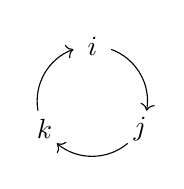
\begin{tikzpicture}[->,scale=.7]
   \node (i) at (90:1cm)  {$i$};
   \node (j) at (-30:1cm) {$j$};
   \node (k) at (210:1cm) {$k$};
%   \node (l) at () {$l};
%   \node (m) at () {$m};

   \draw (70:1cm)  arc (70:-10:1cm);
   \draw (-50:1cm) arc (-50:-130:1cm);
   \draw (190:1cm) arc (190:110:1cm);
\end{tikzpicture} 
    %\lesson{5}{28 February 2025}{Beginning Chapter 2}

\chapter{Trade in the Modern World}

\section{Foreign Portfolio Investment}
\begin{itemize}
    \item Investment in businesses located outside of Canada through stocks, bonds
    and other financial instruments. 
    \item Allows Canadians to spread out their investments, which is less risky than
    investing in just one area. 
    \item Also providess greater choice and opportunity.
\end{itemize}

Canada has a pretty small percentage of world economy, about 3\%. 
For the S\&P/TSX 60 Index, half of it is weighted in energy and finance. \\
Most of the western world is very conservative in global GDP growth,
as most of us are already there. 

\begin{definition}[Importing]
    To bring products or service into a country,
    for use by another business or for resale.
\end{definition}

Majority of the goods that Canada imports 
come from the United States. 

\begin{definition}[Global Sourcing]
    The process of a company buying equipment, 
    capital goods, raw materials, or services from around the world.
\end{definition}

\begin{definition}[Exporting]
    A good produced in one country that is sold into another 
    country. Seller of such good is an exporter; foreign buyers are importers.
\end{definition}

\begin{definition}[Value Adding]
    The amount of worth that is added to a product at 
    each stage of processing. It is the difference between 
    the cost of the raw materials and the finished goods.
\end{definition}

A value adding process could look like this:
Raw Material (50\$) \(\Rightarrow\) Manufacturing of Good (300\$) \(\Rightarrow\) Retail (500\$)
    \section{Trade Barriers}

\begin{definition}[Tariff]
Tariffs, the most common type of trade barrier, are taxes 
or duties put on imported GT's from another country to influence 
products or economics, raise revenues, or product competitive advantages.
\end{definition}

It is not the consumer that pays for the tariff itself. Rather,
the cost of the tariff is passed onto the conusmer.\\ 

Applied to Trump's tariffs plan between Canada and America:
\begin{itemize}
  \item American companies sell goods to Canadian companies.
  \item A tariff is imposed by the American government onto all imports and exports.
  \item Canadian businesses continue importing American goods, but pass the cost onto the consumer.
\end{itemize}

\subsection{Tariff Winners v. Losers (Pros and Cons)}
\textbf{Winners}
\begin{itemize}
  \item The domestic company collects additional taxes.
  \item Goods from local producers are more competitively priced.
  \item Workers in local companies keep employment.
\end{itemize}
\textbf{Losers}
\begin{itemize}
  \item Goods from foreign producers are now more expensive.
  \item The price of products go up and consumers are forced to pay higher prices.
  \item Workers in foreign companies become at risk.
\end{itemize}

A trade imbalance is not inherently good or bad.
With Canada and America, the latter has significant buying power.

\subsection{Domestic and International Issues with Tariffs}

\subsubsection{Domestic Deadweight Loss}
A tariff generally leads to a \textbf{deadweight loss} 
(an excess loss or burden above the amount actually 
paid in tax) as it decreases aggregate economic 
activity and incomes.

\subsubsection{International Disequilibrium}
A tariff would throw off an established market equilibrium. 
A surplus could occur, forcing sellers to sell at lower prices, 
but what would be guaranteed is a recession.

\subsubsection{Overall Economic Slowdown}
Global economic activity recesses, with less money being paid to 
the American government.

\subsection{Trade Barriers}
Canada is heavily dependent on the United States for their economy.
About a third of Canada's GDP is dependent on exports, 75\% of which 
goes to the United States.

\begin{definition}[Protectionism]
The theory or practice of government policy shielding domestic 
industries from international trade, often through trade barriers such as tariffs.
\end{definition}

\subsection{What Motivates Protectionism?}
\begin{itemize}
    \item Response to "dumping"
    \item Response to chronic trade gap
    \item Employment protection 
    \item Protect "fledgling" infant sectors
    \item Protect key/strategic industries
    \item Raise revenues for the government
    \item Response to a recession/low demand
\end{itemize}

Most important things to focus on are: \textbf{Response to chronic trade gap, 
employment protection, raise revenues for the government.}

\begin{definition}[Trade Embargo]
    A government-imposed ban on trade of a specific product or with a specific country, 
    often declared to pressure foreign governments to change their policies.
\end{definition}

Compared to a sanction, an embargo completely shuts down trade between a country. Russia as a good example.

\begin{definition}[Trade Sanctions]
    Economic action taken by a country to coerce another country to conform to an 
    international agreement or norms of conduct.
\end{definition}

North Korea -- No weapons, commodities, luxury goods, travel, or financial services in or to.

\begin{definition}[Trade Quota]
    Government-imposed limit on the quantity, or in exceptional cases the value, 
    of the goods or services that may be exported or imported over a specified period of time.
\end{definition}


    \section{International Business Practices}

\textbf{TODO: Chapter 2 Review}
\begin{itemize}
    \item Complete review package -- Anki deck and complete notes
\end{itemize}

\begin{definition}[Licensing Agreement]
    An agreement that grants permission to a company to use a product, service,
    brand name, or patent, in exchange for a fee or royalty.
\end{definition}

\begin{definition}[Exclusive Distribution Rights]
    A form of licensing agreement that grants a company the right
    to be the only distributor of a product in a specific area or country.
\end{definition}

This provides monopolistic power to the licensee. 
A good example of this would be through a streaming service 
and sports events, such as the NFL and Prime Video. \\

\begin{definition}[Franchise]
    An agreement granted to an individual or group by a company to use that 
    company's name, services, products, and marketing.
    For a fee, the franchisor provides support to the franchisee in the areas of 
    financing, operations, human resources, marketing, advertising, quality control, etc.
    A good example of this is fast food. If you open a fast food franchise, people will automatically
    come, and have expectations in mind, as advertising, ingredients, and preparation is provided by
    the franchisor.
\end{definition}

\begin{definition}[Joint Venture]
    A common type of international business, in which, a new company with shared ownership is formed 
    by two businesses, one of which is usually located in the country where the new company is established.
\end{definition}

\textbf{Joint Venture v. Merger}
A joint venture is an arrangement between two or more businesses to combine their resources. 
They choose the route of a joint venture agreement to accomplish a specific business task. 
Joint ventures, unlike mergers or acquisitions, are often temporary. Once the specific task is 
complete, the joint venture is dissolved. \\

\begin{definition}[Foreign Subsidiaries]
    Often referred to as a \textit{wholly owned subsidiary}, a 
    branch of a company that is run as an independent entity in a country outside of one 
    in which the parent company is located. \\

    The parent company often sets financial targets, and allows the subsidiary to manage its 
    day-to-day operations, so long as those targets are being met. \\
\end{definition}

\subsection{Foreign investment restrictions}
\begin{itemize}
    \item Canadian law with the greatest impact is the \textit{Investments Canada Act}.
    \item Ensures that all foreign investments are reviewed to determine how they will benefit Canada.
\end{itemize}

\subsection{Standards}
\begin{itemize}
    \item Countries have different standards for products in areas such as environmental protection, voltage, health, and safety.
    \item The ISO (International Organization for Standardization) is a network of standardization 
    groups from over 170 countries established to set quality regulations.
\end{itemize}
    \section{Currency Fluctuations}

\begin{definition}[Exchange Rate]
    The amount of one's currency in relation to the currency of another country.
\end{definition}

The Canadian dollar is often quoted against the US dollar, as both countries 
heavily depend on each other in trade.

\textbf{Winners of a High Canadian Dollar}
\begin{itemize}
    \item Importers (purchased goods are relatively cheaper)
    \item Canadian travellers
    \item Major league sports teams in Canada
\end{itemize}

\textbf{Losers of a Low Canadian Dollar}
\begin{itemize}
    \item Exporters (less demand for their products)
    \item Canadian tourism
\end{itemize}

\begin{definition}[Floating Rate]
    An exchange rate that is not fixed in relation to other currencies.
\end{definition}

The price at which currency with a floating rate is bought and sold fluctuates according to supply and demand.
Most advanced economies use floating rates. (USA, Euro, China, Canada, etc.)

\begin{definition}[Currency Revaluation]
    The \textbf{increase} in value of a currency because the demand for 
    that particular currency is greater than supply.
\end{definition}

\pagebreak

\begin{definition}[Currency Devaluation]
    The \textbf{decrease} in value of a currency because the supply of 
    that particular currency is greater than the demand for it.
\end{definition}

\subsection{Factors Affecting Exchange Rate}
\begin{itemize}
    \item Economic conditions in Canada -- Inflation rate, unemployment rate, GDP, interest rates, etc.
    \item Trading between companies -- The more favorable the terms of trade (comparison of exports to imports), the higher the currency exchange.
    \item Politics -- Political tension and instability or the threat of terrorism decreases the demand for a currency.
    \item Psychological factors -- Historical significance and stability change the way currencies are viewed.
\end{itemize}

\begin{definition}[Hard Currencies]
    Stable currencies, such as the Euro, USD, etc., are easily converted to other currencies on the world exchange markets.
\end{definition}

\begin{definition}[Soft Currencies]
    A currency belonging to a country an economy that is small, weak, or fluctuates often, and is difficult to convert, such as the Russian Ruble.
\end{definition}
    \chapter{Culture in International Business}

\section{What is Culture?}

\begin{definition}[Culture]
    Culture encompasses the knowledge, experience, beliefs, values, 
    attitudes, religion, arts, symbols, and possessions acquired by a group 
    of people over time.
\end{definition}

Some aspects of culture can be transmitted through education or by example from one generation to the next.

\begin{definition}[Subculture]
    A cultural group within a larger or predominant culture, distinguished by class, 
    ethnic background, religion, or lifestyle. Generally unified by shared beliefs and interests,
    and are not limited to immigrant populations; you can see subcultures that aren't defined by 
    one's country or origin everywhere.
\end{definition}

\begin{definition}[Counterculture]
    A culture that has values or lifestyles that oppose mainstream values and attitudes,
    usually with a view to challenge the existing norms of a prevailing society.
\end{definition}

\subsection{Canada as a multicultural nation}
\begin{itemize}
    \item Encourages and supports hundreds of different cultural groups within the overall Canadian cultural fabric.
    \item Multiculturalism as \textbf{cultural mosaic}: each of the different cultural groups exists independently as a seperate "tile" that makes up the whole picture.
\end{itemize}

\subsection{Melting Pot v. Salad Bowl}

The melting pot theory requires that immigrants assimilate in order to become one common culture. America and what it means to be American as a good example. \\ 

The salad bowl theory basically calls for us to celebrate our diversity along with our oneness. Canada and being Canadian as a good example.

\section{Business Cultures around the World}

\begin{itemize}
    \item Different countries have very different cultures shaped by various factors.
    \item Business cultures also vary greatly place to place.
    \item Anyone working in international business needs to understand and respect these differences.
    \item \textbf{Cultural intelligence:} the capability to adapt, relate, and work effectively across various culutres. 
\end{itemize}

DONE
    \section{Cultural Awareness and International Business}

\subsection{Doing Business in or with Other Countries}

\begin{itemize}
    \item When cultural differences exist, businesses must decide whether and to what extent its products and processes can be adapted to a foreign environment.
    \item Developing cultural awareness is not an easy task, but it
    is critical to a business’s success in a foreign country.
\end{itemize}

\subsection{Factors that Affect Doing Business Internationally}

\begin{itemize}
    \item Control of foreign operations
    \item Extent of foreign operations 
    \item Number of foreign operations
    \item Degree of cultural difference
\end{itemize}

\subsubsection{Impact on Indigenous Peoples}

\begin{itemize}
    \item When companies set up factories, distribution centres, retail
    stores, or other types of businesses in foreign countries,
    they must be aware of their effect on Indigenous culture.
    \item Effects can be positive (e.g., increased infrastructure,
    employment) or negative (e.g., occupation and destruction
    of lands, disrespect of cultural differences)
    \item A long history of negative impact of industry on Indigenous
    peoples across the globe, including Canada
\end{itemize}


    \section{Impact of Culture on International Business}

\begin{itemize}
    \item Culture’s role in a business venture can be as
    important as the influence of tariffs, legal
    regulations, or competition.
    \item Failure to consider culture could ruin a negotiation,
    derail a marketing campaign, cause labour unrest,
    or, in some cases, endanger one’s life.
\end{itemize}

\subsubsection{Products and Services}
\begin{itemize}
    \item Consider cultural differences to understand what
    products or services will be successful in other
    markets.
    \item Example: Canadian pork cannot be sold in Islamic countries.
    \item Example: Money and Banking \(\Rightarrow\) Saving vs. Spending
    \begin{itemize}
        \item Japan \(\Rightarrow\) Coming of Age
        \item Pilgrimages, weddings, education, etc.
    \end{itemize}
\end{itemize}

\subsection{Culture and the Labour Market}
\begin{itemize}
    \item Consider the impact of and on labour markets in other countries.
    \item \textbf{Rationalization} includes any attempt to increase a company's effectiveness or efficiency.
    \item E.g., \textit{downsizing}, \textit{cutbacks}, and \textit{layoffs}; relocating corporate functions and activities to countries that have cheaper labour.
\end{itemize}

\subsection{Child Labour and Discrimination}
Child labour is prevalent in many countries, and a cultural norm in some, exploitation is common.
On discrimination, while Canada has laws protecting discrimination, it is often difficult to prove, 
and discrimination can be made on other bases.

\subsection{Standards, Practices, and Wages}
Labour unions, vacation entitlement, accommodations like prayer, benefits, etc.
Minimum wage is not the same in all countries, and many countries do not have a fair minimum wage.

\subsection{Business Meetings and Negotiations}
Consider different styles of meetings and negotiations across cultures.
Time perception differs among cultures, with different characteristics. \\ 

Monochronic Cultures have:
\begin{itemize}
    \item Prompt beginnings and endings
    \item Scheduled breaks
    \item Deal with one agenda item at a time
    \item Rely on specific, detailed, and explicit communication
    \item Participants talk in sequence
    \item Lateness is viewed as showing a lack of respect
\end{itemize}

Whereas Polychronic Cultures have:
\begin{itemize}
    \item Flexible start and end times
    \item Breaks happen when appropriate
    \item Don't follow a rigid agenda 
    \item Often deal in broad concepts
    \item Anyone with ideas might speak
    \item Tardiness is not taken personally
\end{itemize}


    % end lessons
\end{document}
